%Einleitung ueber Chaos und Lyapunov Exponent

\section{Ensemble Prediction}
\subsection{The Atmosphere's Chaotic Nature}

%Introduction to the Theory of Stability Buch zum Nachschalgen
%wichtigkeit vohrersagrbarkeit und zuverlaessigkeit qunatifizieren
\citeauthor{poincare1897forme} was the first one to describe a chaotic system, namely the solar system. When he tried to predict the planetary orbits, he started with the simplest case, a system of two large bodies, rotating each other, and discovered that even a very small third body can destabilize the system  \cite{poincare1897forme}.
Then a long time passed, before Edward Lorenz, who is often referred to as the father of chaos theory, published his discovery, revealing why the difficulties of reliable meteorological forecasts are inherent:
Atmospheric dynamics is highly sensitive to even the smallest changes in the initial and boundary conditions. A small error can propagate and be amplified through non-linear feedback processes to a magnitude much higher than its initial value. If that is the case, completely different scenarios emerge after some time \cite{lorenz1963deterministic}. This behaviour is called chaotic and in context of atmospheric motions broadly known as `Butterfly Effect'. The name origins in one of Lorenz' most famous talks, where he illustrated his complex theory with the question `Does the flap  of a butterfly's  wings in Brazil set off a tornado  in Texas?', discussing the immense effects of extremely small changes in the initial conditions of an atmospheric state on the occurrence of extreme weather events and general predictability of future atmospheric states \parencite{lorenz2000butterfly}. 

A more thorough mathematical definition of chaos is provided by the Lyapunov-exponents, which are briefly described in the following after \citeauthor{kalnay2003atmospheric} \cite{kalnay2003atmospheric}.\\ \\
In general, all possible states of a dynamical system, that can be described by $n$ independent variables $x_{1}, \ ... \ , x_{n}$ can be represented by the system's $n$-dimensional phase space $\Gamma$.
A volume in phase space is defined by a set of states $\vec{x}=(x_{1}, ... , x_{n}) \in \Gamma$. To illustrate this, we use the example of the states contained in a hypersphere $\Gamma_{S}$ with a set radius $r$

\begin{equation}
    \Gamma_{S} = \{ \vec{x}:|| \vec{x}||\leq r \} \quad .
\end{equation}
Then a volume $V$ can be assigned to the set by using the indicator function $f$ of the set $\Gamma_{S}$ and the Liouville measure $d\vec{x}=dx_{1}dx_{2}...dx_{n}$
\begin{equation}
    V = \int_\Gamma f d\vec{x} \quad .
    \label{eq:volps}
\end{equation}
This phase space volume $V$ can be used to determine, whether a system can be described by Hamiltonian mechanics, or if it is necessary to move to the more complex framework of dynamical system theory, including chaos theory.
The criterion for a system to be Hamiltonian, is that any initial phase space volume is conserved \cite{knauf2018linear}. \\
Let us now consider a point in phase space and apply an initial spherical infinitesimal perturbation to the point as illustrated in Figure \ref{fig:phasespace}. Then, the evolution of the sphere in time can be used to categorize the system. 
\begin{figure}[h]
      \captionsetup{width=.8\linewidth}
    \centering
    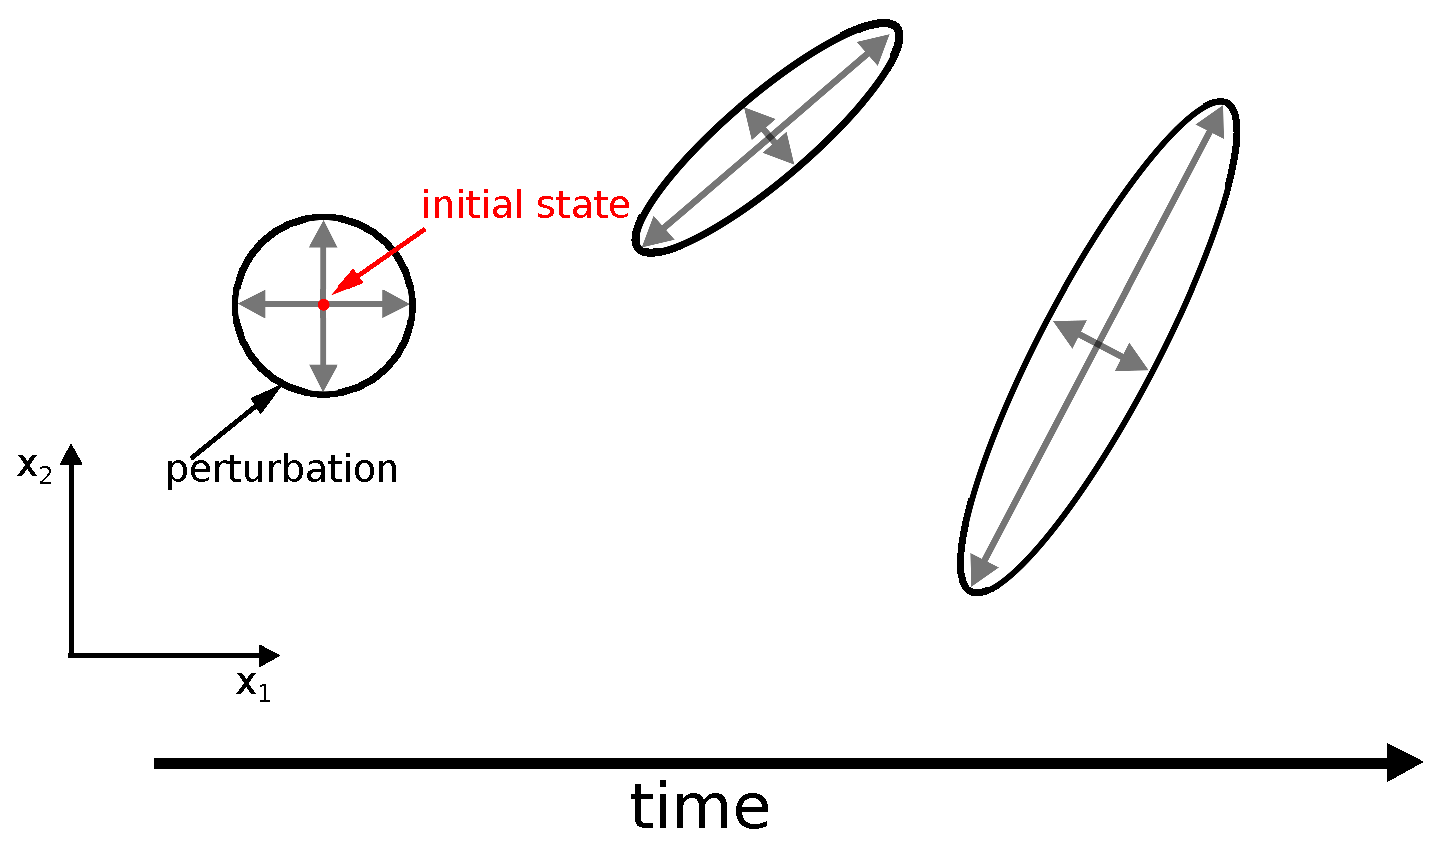
\includegraphics[width=0.8\textwidth]{graphics/phasespace_deform.eps}
    \caption[Deformation of Phase Space Volume]{Example of a deformation of a volume in a two-dimensional phase space: the red dot marks the deterministic initial state and the sphere the initial perturbation. The phase space volume of  the initially spherical perturbation is deformed with respect to the stability properties of the dynamical system \cite{kalnay2003atmospheric}.}
    \label{fig:phasespace}
\end{figure}
The deformation of the sphere is determined by its axes $a_{1}, \  ..., \ a_{n}$. The axes describe the separation rates of the trajectories, that started infinitesimally close. A parameter $\vec{\lambda} = (\lambda_{1},  ... ,\lambda_{m})$ is introduced so that any axis becomes the initial length scaled by $\lambda_{j}$ after a time $t$
\begin{equation}
    a_{i}(t) = a_{i}(0) e^{\lambda_{j}t} \quad ,
\end{equation}
resulting in a deformation of the volume of the sphere
\begin{equation}
    V(t) = V(0) \ e^{-\sum^{m}_{j=1} \lambda_{j}t} \quad .
\end{equation}
The coefficients $\lambda_{j}$  are called Lyapunov-exponents and their indices denote their relative magnitude:
\begin{equation}
  \forall  \lambda_{j}:\lambda_{j} \geq  \lambda_{j+1} \quad .
\end{equation}
Then the condition for a Hamiltonian system of the conservation of the initial volume of the sphere in phase space can be expressed as:
\begin{equation}
    \sum^{m}_{j=1}\lambda_{j} =0 \quad
\end{equation}
the condition for a stable system:
\begin{equation}
     \forall  \lambda_{j}:\lambda_{j} \leq 0
\end{equation}
and the condition for a chaotic system:
\begin{equation}
    \exists  \lambda_{j}:\lambda_{j} > 0 \quad .
\end{equation}
As those conditions imply, the volume contained in the sphere is conserved or can even converge to a point for a stable system. For a chaotic system at least $\lambda_{1}$ has to be greater than zero, so that trajectories in phase space diverge. In the textbook by \citeauthor{kalnay2003atmospheric} \cite{kalnay2003atmospheric} the meaning of the Lyapunov-exponents is summarized as the following: `[...]the Lyapunov-exponents describe the long-term average exponential rate of stretching or contraction in the attractor.'. The term attractor is used for the set of points that the trajectories pass multiple times.\\
For a stable system, reliable forecasts can be done at all times, where on the other hand, chaotic systems become unpredictable after a finite time. The Lyapunov-exponents and hence, the predictability of a system, can be calculated from theory or from experimental data \parencite{eckmann1986liapunov, vannitsem2017predictability, leutbecher2008ensemble}.



\subsection{Ensembles}

Since the beginning of the 1990s  ensemble prediction has become a widely-known approach to treat uncertainty in NWP and it is still considered state of the art and subject of current research with increasing popularity \cite{wilks2011statistical, bauer2015quiet, leutbecher2008ensemble, Shemyakin2018,palmer1993ensemble}. 
To estimate the effect of different values for the initial and boundary condition and model parametrizations  a so-called ensemble is created.
Each ensemble member represents a different simulation. It is a single trajectory in the phase space of the atmospheric system. For traditional ensembles independent runs for all members are performed and the statistical properties of the whole ensemble data set are evaluated \cite{leutbecher2008ensemble}.\\
There are three main types of ensembles:
\begin{enumerate}
\item {Multi-model ensemble: Each member uses a different NWP model  \cite{ebert}}
\item{Multi-physics ensemble: Each member uses different parametrizations or different settings of the model physics \cite{Houtekamer}}
\item{Traditional ensemble: Each member is obtained by perturbing one or more quantities in initial or boundary conditions, or in the model itself. If random number sampling is used, it is called Monte-Carlo forecast.}
\cite{du2007uncertainty, wilks2011statistical, leith1974theoretical}
\end{enumerate}
Figure \ref{fig:ecmwf_ensemble} shows an example of a traditional ensemble forecast and its components: ensemble forecasts contain several regular members and a control member, which is the deterministic scenario (the scenario considered most likely), with the same resolution as the other ensemble members. In most cases, the deterministic run is performed with a higher resolution, to get the best possible forecast. Unfortunately it would consume too much computational resources to run the whole ensemble on the highest possible resolution. Thus, a control member is computed additionally, to have a point of reference for the other ensemble members without the bias of different resolutions.\\
Depending on the type and source of uncertainty we want to investigate, we need to create an appropriate ensemble.\\
\begin{figure}[H]
    \centering
    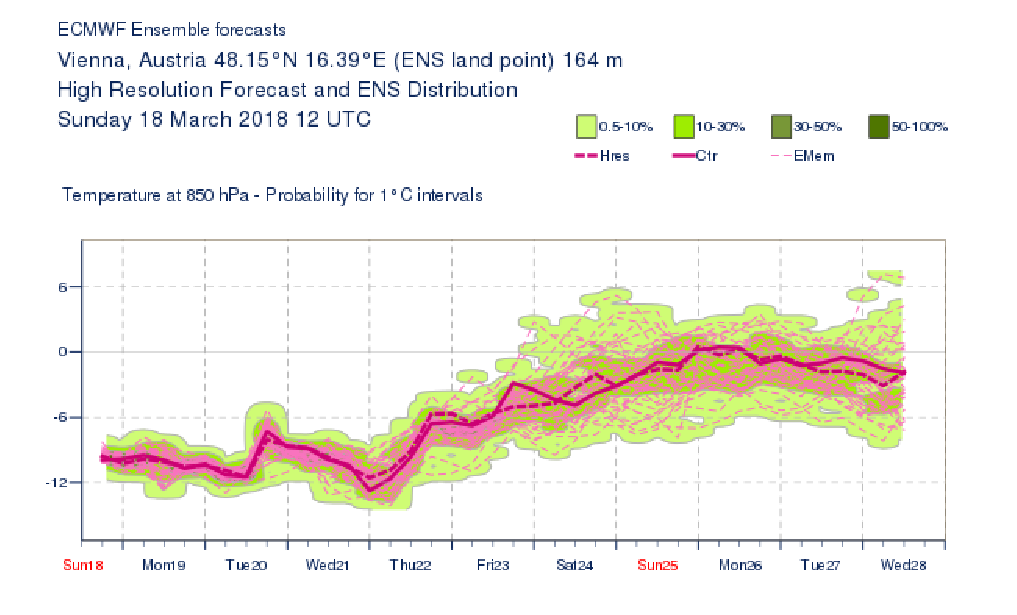
\includegraphics[width=0.8\textwidth]{graphics/ecwmfensemble_clip.eps}
    \caption[Example of Ensemble Forecast]{ECMWF ensemble: A temperature ensemble forecast of the ECMWF showing 50 regular members (`EMem'), one control member (`Ctr') and one high resolution run (`Hres'). The ensemble spread increases with time, revealing the chaotic dynamics of the atmosphere. The number of  ensemble members in a certain temperature interval can be related to the probability of a certain temperature. The image was created by the ECMWF (cannot be accessed by the public).}
    \label{fig:ecmwf_ensemble}
\end{figure}
In this study we focused on ensemble creation by stochastically perturbed parameters, a Monte-Carlo method, which is explained in greater detail in Subsection \ref{sec:Monte}.

\subsection{Uncertainty and Error}

The sources of error can be categorized into three groups: initial conditions, model error and, for limited area models (LAM), boundary conditions.
The initial conditions of the model equations have a very high level of uncertainty. Many of them are set by a best-guess gained from old model output combined with new measurements. But the number of measurement stations is usually small in comparison to the number of grid points in a model and also the measurement equipment has a limited accuracy. It is worth pointing out, that the problem is not only about the difference in number of grid points and measurement stations but also that the locations of grid points and measurement stations do not overlap. \\
The boundary conditions for limited area models are even more sensitive, because they are set to the output values obtained from a global model. Thus, errors can evolve and be amplified in the global model and are then passed on to the LAM, especially affecting the forecast quality on the edges of the domain.\\
A consequence of the limited resolution of the model is that many processes, that take place on a sub-grid scale, have to be parametrized.
Since every parametrization is an approximation, all parametrized physical processes contribute to the uncertainty in a model \cite{leutbecher2008ensemble}.
Even if a physical process is resolved explicitly, it contributes to model error, due to the model being discrete. In nature, on the other hand, most of the concerned processes evolve continuously on the model's scales. 
Another source of uncertainty is that for some quantities in the model, like aerosol concentration, only climatological data is used. The reason being, that  prognostic schemes require too much computational resources and/or there is a lack of up-to-date data. \\
A problem specific to NWP models is the orographic mismatch. Especially in mountainous regions not all topographic structures can be resolved. This can cause a large discrepancy between reality and model.\\

\subsection{Ensemble Creation by Monte-Carlo Methods}
\label{sec:Monte}
In a stochastic ensemble, each member represents a different possible value of a certain quantity. How the values differ for the members is determined by a random sampling regime. Ensemble members are created by perturbing a deterministic value, that we will call the unperturbed value from now on. But it is important to acknowledge that the unperturbed value shall never be seen as the `real' value of a variable, but the most likely value. A value being categorized as most likely can be based on climatological data, knowledge of the underlying physics or current measurement data. Because of limited accuracy of measurement equipment and the spatial resolution, it is inherently impossible to determine a `real' value of a variable in an atmospheric system. Only a certain range for the values can be determined. \\
We distinguish the different perturbation schemes by the perturbed quantity:
\begin{enumerate}
    \item {Perturbing the initial value of a variable}
    \item {Perturbing the tendency of a variable (SPPT)}
    \item {Perturbing constant parameters in a parametrization (SPP)}
\end{enumerate}
The SPPT and the SPP perturbation schemes are used to take model error into account. Perturbation of the initial values, on the other hand,  incorporates the errors contributed by the set-up of initial and/or boundary conditions.\\
The different schemes are briefly outlined in the following. 

\subsubsection{Perturbation of initial conditions }
The simple random perturbation of initial conditions is the most basic perturbation scheme.
Let $e_{j}$ be the time integration of the model equations (`prognostic variable')
\begin{equation}
    \frac{\partial e_{j}}{\partial t} = A(e_{j},t) + P(e_{j},c_{0},..., c_{N}) \quad ,
    \label{eq:icpert1}
\end{equation}
where $A$ are the non-parametrized and $P$ are the parametrized contributions, which depend on $e_{j}$, the time $t$ and $N$ constant parameters $c_{0},..., c_{N}$.\\
Now only the initial conditions are perturbed
\begin{equation}
    e_{j}(t=0) \equiv e_{j,0}+ \delta e_{j}(t=0) \quad ,
    \label{eq:icpert2}
\end{equation}
where $ e_{j,0}$ is the deterministic value at $t=0$ and $\delta e_{j}$ is the  perturbation.
From investigation of  Equation \eqref{eq:icpert1} and \eqref{eq:icpert2} it is obvious that the difference in the evolution of different ensemble members has its origin solely in the perturbation of initial conditions. The simplest way to set-up the perturbation is to only perform random sampling. But today more sophisticated techniques, like the use of Lyapunov-exponents, are more common than a plain Monte-Carlo approach \cite{0034-4885-63-2-201, buizza1999stochastic}.

\subsubsection{Stochastically Perturbed Parametrized Tendencies (SPPT)}
In the model equations the tendencies of all model variables are calculated at each time step and used for the integration. The tendency of a variable is defined as its change in one time step. It is the sum of the change of the variable calculated from the Primitive Equations $A(e_{j},t)$ and the change contributed by parametrized processes $P(e_{j},c_{0},..., c_{\mathrm{N}})$. Thus, $P(e_{j},c_{0},..., c_{\mathrm{N}})$ is called  parametrized tendency hereafter.
We start as before, but now the parametrized tendency $P$ is perturbed and denoted by $P^{\prime}$
\begin{equation}
    \frac{\partial e_{j}}{\partial t} = A(e_{j},t) + P^{\prime}(e_{j},c_{0},..., c_{\mathrm{N}}) \quad .
    \label{eq:sppt}
\end{equation}
For each grid point the perturbed parametrized tendency is defined as
\begin{equation}
   P^{\prime} \equiv r_{j}(\lambda_{\mathrm{lon}}, \phi, t) P \quad ,
\end{equation}
where $ r_{j}$ is a random number. It is taken from a spatially and temporally correlated pattern consisting of randomly sampled numbers, chosen from a suitable distribution \parencite{buizza1999stochastic}. Regarding Equation \eqref{eq:sppt}, it is noteworthy that only errors contributed by parametrizations are considered.


\subsubsection{Stochastically Perturbed Parameters (SPP)}
We start as before, but now the constant parameters $c_{0},..., c_{\mathrm{N}}$ in the parametrized tendency $P$ are perturbed. Therefore the resulting parametrized tendencies are denoted by $P^{\prime \prime}$ 
\begin{equation}
    \frac{\partial e_{j}}{\partial t} = A(e_{j},t) + P^{\prime \prime}(e_{j},c_{0}r_{0},..., c_{\mathrm{N}}r_{\mathrm{N}}) \quad .
\end{equation}

For each grid point the perturbed parametrization is defined as
\begin{equation}
   P^{\prime \prime} \equiv  P^{\prime \prime }(e_{j}, c_{0} r_{0}(\lambda_{\mathrm{lon}}, \phi, t), ..., c_{\mathrm{N}} r_{\mathrm{N}}(\lambda_{\mathrm{lon}}, \phi, t)) \quad ,
\end{equation}
where again, $ r_{j}$ is a random number, taken from a spatially and temporally correlated
pattern consisting of randomly sampled numbers. In this regime the uncertainties can be directly related to single physical parameters \parencite{ollinaho2017towards}.\\ \\

The choice of scheme depends on what we want to examine and how the sources of error should be weighted.

For example, if we want to investigate the effect of the variation of initial conditions due to limited accuracy in measurements and hence, in data assimilation, then the initial value of the variable needs to be perturbed.
To examine the effects of uncertainty due to model error, introduced by spatial and time discretization, the tendencies of the variables should be perturbed as well. There are many parametrized processes contributing to the tendencies, so perturbing the tendencies can be an effective way to increase model spread based on acknowledging the effect of uncertainties in different parametrizations.\\

If we obtained a parametrization e.g. by fitting data, then, to analyse the impact of the uncertainty of the coefficients, the constant parameters can be perturbed.

To decide which variables, parameters or tendencies should be perturbed, one has to identify those, which have the highest level of uncertainty and which are most influential to the model output. Moreover, one must consider what is computationally affordable and stable.\\


